\documentclass[10pt]{article}
%\documentclass[10pt]{scrartcl}
%T \usepackage{newtxtext,newtxmath}
\usepackage{url}
\usepackage{pcsjimps-e}
\usepackage[dvipdfmx]{graphicx}
\usepackage[dvipdfmx,bookmarks=false]{hyperref}

\begin{document}
\pagestyle{empty}

\twocolumn[\centering
% Title
\ETitle{
How to Prepare a Camera-Ready Paper for Picture Coding Symposium of Japan and
Image Media Processing Symposium}

% Author names
\EAuthor{Author 1$^\dag$}{70mm}
\EAuthor{Author 2$^\ddag$}{70mm}\\

% Affiliation
\EAffiliation{$^\dag$PCSJ/IMPS Organizing Committee}{70mm}
\EAffiliation{$^\ddag$English Affiliation 2}{70mm}\\

% Abstract
\Abstract{
English abstract (about 100 words). 
English abstract English abstract English abstract English abstract 
English abstract English abstract English abstract English abstract 
English abstract English abstract English abstract English abstract 
English abstract English abstract English abstract English abstract 
English abstract English abstract English abstract English abstract 
English abstract English abstract English abstract English abstract 
English abstract English abstract English abstract English abstract 
English abstract English abstract English abstract English abstract 
English abstract English abstract English abstract English abstract 
English abstract English abstract English abstract English abstract 
English abstract English abstract English abstract English abstract 
}
]


\section{Introduction}

The proceedings is published in USB media and printed material 
(monochrome). Please submit your manuscript electronically in PDF format.

The manuscript for invited/special talks has less page limit (up to 8 
pages) and in free format. A photograph and biography of the lecturer 
are presented in its first page.

This sample is aimed at the manuscript for \underline{ordinary 
presentations}.


\vspace{5cm}

\section{Length and Typeset Parameters}

\begin{itemize}
\item up to two pages including figures and tables
\item A4 size
\item text area width of 180mm
\item text area height of 252mm
\item baseline skip of 8mm
\end{itemize}

\vspace{5cm}

\section{Format Outline}

\begin{itemize}
\item abstract of about 100 words
\item manuscript can be either one-column or two-column.
\item put the contact information at the bottom-right of the 
      last page. (You may want to use sample macro \verb|\simplefootnotetext|).
\end{itemize}


\vspace{5cm}

\section{Font Sizes}

Following font sizes are recommended.
\begin{description}
\item[Title] 16pt (\verb|\LARGE|)
\item[Author names] 12pt(\verb|\large|)
\item[Affiliation and text] 10pt(\verb|\normalsize|)
\end{description}


\vspace{5cm}

\section{Tables and Figures}

\begin{table}[tb]
\caption{Encoder Settings.}
\label{tab:settings}
\centering
\begin{tabular}{c||c|c}\hline
 configuration 1 & aa & aaa\\\hline
 configuration 2 & bb & bbb\\\hline
 configuration 3 & cc & ccc\\\hline
\end{tabular}
\end{table}

\begin{figure}[tb]
\centering
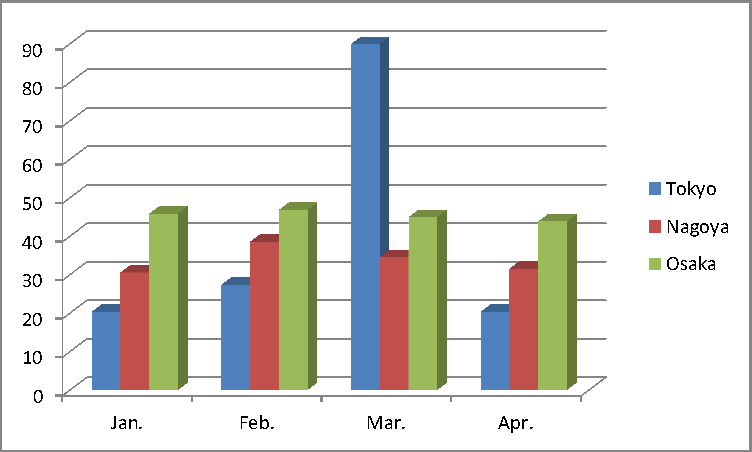
\includegraphics[width=.55\columnwidth]{sample-e.eps}\\
\caption{Coding results.}
\label{fig:results}
\end{figure}

Please be aware that your manuscript will be printed in monochrome, 
halftone dot meshing.

Figures and tables shall be placed at the top or bottom of a column wherever possible.
For \TeX floats, the placement parameter shall be either [t] or [b]. [h] shall be 
used sparingly, or not at all.
Refer to them with e.g., 
\figref{results} and \tabref{settings}.

\vspace{5cm}

\section{Creating a PDF File}
Please be sure to embed all the fonts when creating a PDF file.
Double check to see if the fonts are embedded in the created PDF file 
with Acrobat or some free tools.

Examples of PDF creation command are:
\begin{verbatim}
$ latex foo.tex
$ dvipdfmx -p a4 foo.dvi
or
$ simpdftex latex --mode dvipdfmx --dvipdfmopts \
  "-p a4" foo.tex
\end{verbatim}

\vspace{5cm}

\section{Other \LaTeXe-Specific Tips}

You may use newtx\cite{newtx} package etc. to have more beautiful typesetting.

%T \def\egstr{{\it Font Example}, Bj\o ntegaard delta, {\it Karsten S\"uhring}}
%T Following examples are with Times-Roman font of txfont
%T and with normal \TeX\ font (Computer Modern Roman):\\
%T \egstr\\
%T {\renewcommand{\rmdefault}{cmr}\normalfont \egstr}

To show URLs, consider the use of url style file with \verb|\url{http://...}|.

You may use 
hyperref package\cite{hyperref} to 
build a PDF file that contains hyperlink information. 

\vspace{5cm}

\section{Conclusion}
2014.05.13 Initial Version\\
2015.07.15 Revised Version


\def\etal{{\it et al.}}
\begin{thebibliography}{9}
 \bibitem{CALIC} X. Wu \etal: ``Context-based, adaptive, 
	 lossless image codec,'' IEEE Trans. Commun., vol. 45, pp. 437--444, 
	 Apr. 1997
 \bibitem{newtx}
	 M. Sharpe: ``newtx -- Alternative uses of the TX fonts, with improved metrics'',
	 available at \url{http://www.ctan.org/pkg/newtx}
 \bibitem{hyperref}
	 \url{https://en.wikibooks.org/wiki/LaTeX/Hyperlinks}
\end{thebibliography}

\simplefootnotetext{
ABC Department, XYZ Laboratories\\
Street address, City, Zip\\
Phone: 000-111-2222, Fax: 000-111-2223\\
E-mail: foo@example.edu}
\end{document}
